\documentclass[journal,twoside]{IEEEtran}
\usepackage{cite}
\usepackage{amsmath,latexsym,amssymb,amsfonts}
\usepackage[utf8]{inputenc}
\usepackage{textcomp}
\usepackage[dvipsnames]{xcolor}
\usepackage{booktabs}
\usepackage{graphicx}
\usepackage{url}
\usepackage{hyperref}
\usepackage{bm}
\usepackage{amsthm}

%%%%%%%%%%%%%%%%%%%%%%%%%%%%%%%%%%%%%%%%%%%%%%%%%%%%%%%%%
\usepackage{tikz}
\usetikzlibrary{circuits.ee.IEC}
\usepackage[european resistor, european voltage, european current]{circuitikz}
\usetikzlibrary{arrows, shapes, positioning}
\usetikzlibrary{decorations.markings, decorations.pathmorphing,
decorations.pathreplacing}
\usetikzlibrary{calc,patterns,shapes.geometric}
\usetikzlibrary{shapes.multipart, positioning, patterns, backgrounds}
\tikzstyle{titlebox}=[rectangle,inner sep=10pt,inner ysep=10pt,draw]%
\usetikzlibrary{arrows.meta}
\usetikzlibrary{matrix, fit}

%%%%%%%%%%%%%%%%%%%%%%%%%%%%%%%%%%%%%%%%%%%%%%%%%%%%%%%%%%%%%

\def\blacksquare{\hbox{\vrule width 4pt height 4pt depth 0pt}}
\def\square{\hbox{\vrule width 4pt height 4pt depth 0pt}}
\def\qed{\hfill \square}
\def\qedp{\rightline{$\blacksquare$}}
\def\EXPT{\mathop{{\rm E}}}
\def\MIN{\mathop{{\rm min}}}
\def\MAX{\mathop{{\rm max}}}
\def\LIM{\mathop{{\longrightarrow}}}
\def\UNION{\mathop{\bigcup}}
\def\INTERSECT{\mathop{\bigcap}}
\def\ARGMIN{\mathop{{\rm argmin}}}
\def\ARGMAX{\mathop{{\rm argmax}}}
\def\TOUND{\mathop{\longrightarrow}}
\def\col#1{\mathop{{\rm col}\,\left(\,#1\,\right)}}
\def\rank{\mathop{{\rm rank}}}

\newcommand{\widebox}[2][0.5em]{\fbox{\hspace{#1}$\displaystyle #2$\hspace{#1}}}

% User definition from Shengya
\def\V{\mathcal{V}} % the set of vehicle
\def\E{\mathcal{E}} % the set of edge
\def\G{\mathcal{G}} % graph
\def\A{\mathcal{A}} % adjacency matrix 
\def\W{\mathcal{W}} % weighted adjacency matrix
\def\L{\mathcal{L}} % Laplacian matrix
\def\N{\mathcal{N}} % neighbors
\def\LO{\mathcal{LO}} % the set of observer
\def\DO{\mathcal{DO}} % the set of observer
\def\diag#1{\mathop{{\rm diag}\,\left(\,#1\,\right)}}
\def\ST{\mathcal{ST}} % Self trust
\def\LT{\mathcal{LT}} % Local trust
\def\DT{\mathcal{DT}} % Distributed trust 
\def\VT{\mathcal{VT}} % Vehicle trust 
\def\AT{\mathcal{AT}} % Aggregation trust
\def\T{\mathcal{T}} % Aggregation trust
\def\O{\mathcal{O}} % opinion


% User Defined Color based on RGB
\definecolor{userblue}{RGB}{31,119,180}
\definecolor{userorange}{RGB}{255,127,14}
\definecolor{usergreen}{RGB}{44,160,44}
\definecolor{userpurple}{RGB}{148,103,189}

\definecolor{blue1}{RGB}{31,119,180}
\definecolor{orange1}{RGB}{255,127,14}
\definecolor{green1}{RGB}{44,160,44}
\definecolor{purple1}{RGB}{148,103,189}
\definecolor{rose1}{RGB}{227, 119, 194}

%%%
\newtheorem{prb}{\it Problem}%[section]
\newtheorem{theorem}{\it Theorem}%[section]
\newtheorem{lemma}{\it Lemma}%[section]
\newtheorem{definition}{\it Definition}
\newtheorem{remark}{\it Remark}%[section]
\newtheorem{assumption}{\it Assumption}%[section]
\newtheorem{example}{\it Example}%[section]
\newtheorem{annex}{\it Annex}%[section]
\newtheorem{prop}{\it Proposition}%[section]

\newtheorem{alert}{\color{red}\it Alert Remark}
% \newtheorem{proof}{\it Proof}%[section]




\def\BibTeX{{\rm B\kern-.05em{\sc i\kern-.025em b}\kern-.08em
    T\kern-.1667em\lower.7ex\hbox{E}\kern-.125emX}}

\tikzset{global scale/.style={
    scale=#1,
    every node/.append style={scale=#1}
  }
}

\begin{document}

\title{Trust-Aware Resilient Distributed Observer Design for Connected Vehicle Platoons}
\author{Q.H. Nguyen, Shengya Meng, H. Rafaralahy, M. Haddad, and A. Zemouche%
\thanks{This work was supported by SEGULA Engineering. H. Rafaralahy and A. Zemouche acknowledge the ANR agency for its partial financial support under project ArtISMo ANR-20-CE48-0015.}%
\thanks{Q.H. Nguyen, Shengya Meng, H. Rafaralahy, and A. Zemouche are with Universit\'e de Lorraine, CNRS, CRAN, F-57000 Metz, France (e-mail: ali.zemouche@univ-lorraine.fr).}%
\thanks{Q.H. Nguyen and M. Haddad are with SEGULA Engineering, 19 rue d'Arras, 92000 Nanterre, France (e-mail: madjid.haddad@segula.fr).}%
\thanks{QCar/LIMO implementation resources are available at \protect\url{https://github.com/kslhuy/QCar2_Cran}.}}

\markboth{IEEE Transactions on Vehicular Technology,~Vol.~XX, No.~XX, 2026}{Nguyen \MakeLowercase{\textit{et al.}}: Trust-Aware Resilient Distributed Observer Design}
\maketitle

\begin{abstract}
Connected vehicle platoons depend on distributed state estimation, but vehicle-to-vehicle data can be corrupted by falsified states, replayed or delayed packets, packet drops, and compromised vehicles. This paper proposes a trust-aware resilient distributed observer for vehicles described by a discrete kinematic bicycle model. The observer converts local and distributed consistency checks into online observer weights. The resulting observer builds a time-varying trusted-neighbor set while preserving a local-observer anchor, so unreliable data are down-weighted without discarding useful cooperation from reliable vehicles. Sufficient input-to-state stability conditions are derived for bounded model uncertainty, input mismatch, linearization remainders, and trust-induced switching along bounded trajectories. A finite-window rollback mechanism is also formulated to mitigate contamination caused by delayed trust decisions. Simulations on a four-vehicle platoon under position, speed, heading, input, and packet-drop attacks show bounded estimation degradation; in the tested closed-loop attack interval, the trust-modulated IDM/CACC controller preserves positive inter-vehicle spacing through longitudinal projection.
\end{abstract}

\begin{IEEEkeywords}
Connected vehicles, cyber-physical systems, distributed observers, secure state estimation, trust management, vehicle platooning.
\end{IEEEkeywords}

\section{Introduction}\label{sec_introduction}
\IEEEPARstart{C}{onnected} and automated vehicle platoons rely on vehicle-to-vehicle (V2V) communication to coordinate longitudinal motion, improve traffic throughput, reduce fuel consumption, and maintain safe inter-vehicle spacing. In this setting, each vehicle must estimate not only its own state but also the states of surrounding platoon members from a mixture of onboard sensing and communicated information. This distributed estimation layer is therefore a critical component of cooperative adaptive cruise control and other platoon-level decision loops.

The same communication structure that enables cooperation also creates a vulnerability: falsified, delayed, replayed, or missing packets can corrupt local and distributed estimates. Conventional distributed observers often assume that exchanged data are reliable, which is restrictive for connected-vehicle applications exposed to cyberattacks, packet drops, and faulty nodes. Once compromised information is accepted by the observer, the resulting estimation error can propagate across the communication graph and degrade both safety and closed-loop performance.

This paper develops a trust-aware distributed observer for resilient platoon state estimation. The main idea is to evaluate the behavioral consistency of received data, convert this consistency into trust scores, and use those scores to adapt the observer weights online. As a result, the observer can reduce the influence of unreliable neighbors while preserving useful cooperation from reliable vehicles. The proposed formulation clarifies the threat model, connects trust evaluation to the ISS analysis, introduces a bounded rollback module for delayed decisions, and evaluates the estimator under multiple communication faults.

The main contributions are summarized as follows:
\begin{itemize}
    \item A resilient distributed state-estimation architecture for connected vehicle platoons under adversarial communication.
    \item A behavioral trust framework that combines local consistency, distributed-estimate consistency, freshness, and temporal smoothing to construct a trusted-neighbor set.
    \item A trust-adaptive observer-weight design with input-to-state stability (ISS) guarantees for bounded modeling, input, and linearization mismatches in the local time-varying bicycle-error model.
    \item A finite-window rollback mechanism that can re-propagate recent observer updates after delayed trust decisions.
    \item Simulation evidence under position, velocity, heading, input, and packet-drop attack cases, together with a closed-loop spacing check during the attack interval using the current IDM/CACC structure through path-longitudinal projection.
\end{itemize}

The remainder of the paper is organized as follows. Section~\ref{sec_related_work} reviews related work and motivates the proposed approach. Section~\ref{sec_vehiclemodel} introduces the graph notation, vehicle model, and threat model. Section~\ref{sec_distributed_observer} presents the distributed observer architecture. Section~\ref{sec_trust_score} defines the trust framework. Section~\ref{sec_weight_design} develops the trust-based weight design and stability analysis. Section~\ref{sec_rollback} presents the delayed-decision rollback module. Section~\ref{sec_simulation} reports the simulation study, QCar/LIMO platform implementation, and controller spacing check, and Section~\ref{sec_conclusion} concludes the paper.

\section{Related Work and Motivation}\label{sec_related_work}
Security and resilience for connected vehicle platoons have been studied through attack detection, fault-tolerant estimation, and mitigation-oriented control. Observer-based methods compare model-predicted states with measurements or received data to detect abnormal behavior~\cite{jeon2020simultaneous,yamamoto2021attack,huang2022detection,2_obs_Angelo}. These methods are attractive because they are model-aware and can be implemented locally, but their performance degrades when the observer itself uses corrupted neighbor information.

Consensus and distributed-estimation methods exploit redundancy across multiple agents or sensors~\cite{Guitao_multi_mesure,Consensus_discret_Saber,Plug_play}. They can improve robustness by cross-validating information, but many approaches implicitly require sufficiently reliable neighbors or fixed communication weights. Under coordinated attacks, persistent packet loss, or biased local observers, fixed consensus weights can spread wrong estimates instead of isolating them. More general secure-estimation methods include bank-of-observers selection under sparse sensor attacks~\cite{chong2021secure} and distributed $\ell_1$ state-and-fault estimation for multi-agent systems~\cite{hashimoto2020distributed_l1}; these provide useful resilient-estimation baselines, but they do not directly provide trust-adaptive V2V observer weights for platoons.

Set-membership and data-driven techniques provide another line of resilient estimation and detection. Zonotopic set-based estimators propagate all states consistent with bounded uncertainties and can guarantee true-state containment under time-varying sensor attacks when sufficient uncompromised sensing remains~\cite{niazi2023resilient_set}. Data-driven attack-detection methods instead use attack-free input-output trajectories to identify uncompromised sensors online, including extensions for replay and delay attacks~\cite{coimbatore2025data_driven_attack}. These methods are useful for guaranteed or model-learning-based security analysis, but they are generally centralized or detection-oriented and do not directly adapt the distributed V2V observer weights used by a platoon controller.

Trust-based approaches assign reliability scores to agents or data streams. Physical-layer and connectivity-based methods use signal fingerprints or communication characteristics to authenticate neighbors~\cite{trust_physic_connecte,KF_chisquare_meusure}, while behavior-based methods compare exchanged data with local sensing or expected motion~\cite{trust_simple,trust_complex}. Context-aware IoV trust management further incorporates application context, rational trust-attribute weighting, and adaptive misbehavior thresholds to improve attack resistance in dynamic vehicular networks~\cite{siddiqui2023trust_vehicles}. Trust can also be injected into control policies to reduce the influence of unreliable vehicles~\cite{self-belive,Enhancing_control_trust}. However, these trust mechanisms are usually diagnostic, reputation-oriented, or controller-side filters; they do not directly provide a trust-adaptive distributed observer with stability guarantees and delayed-decision rollback.

The present work is motivated by this gap. Instead of treating trust as an external diagnostic signal, the proposed method feeds trust directly into the observer-weight design. The observer therefore adapts its communication graph online while preserving a local-observer anchor, which improves recoverability after transient attacks and supports a stability analysis for bounded disturbances.

\begin{table*}[!t]
\centering
\caption{Positioning of the proposed method relative to related resilient platoon/state-estimation approaches.}
\label{tab:related_comparison}
\scriptsize
\begin{tabular}{p{2.7cm}p{2.7cm}ccccc}
\toprule
\textbf{Approach} & \textbf{Typical attack class} & \textbf{Dist. observer} & \textbf{Adaptive trust weights} & \textbf{ISS/stability} & \textbf{Rollback} & \textbf{Closed-loop use} \\
\midrule
Observer residual detection~\cite{jeon2020simultaneous,yamamoto2021attack,huang2022detection,2_obs_Angelo} & Sensor/communication anomalies & Partial & No & Case dependent & No & Partial \\
Consensus/distributed estimation~\cite{Guitao_multi_mesure,Consensus_discret_Saber,Plug_play} & Noise and model mismatch & Yes & No & Yes & No & Limited \\
Bank-of-observers secure estimation~\cite{chong2021secure} & Sparse sensor attacks & No (bank) & No & Yes & No & No \\
Distributed $\ell_1$ state/fault estimation~\cite{hashimoto2020distributed_l1} & Sparse faulty agents & Yes & No & Error bound & No & No \\
Set-membership/zonotopic estimation~\cite{niazi2023resilient_set} & Time-varying sensor attacks & No & No & Set inclusion & No & No \\
Data-driven attack detection~\cite{coimbatore2025data_driven_attack} & Sensor, replay, delay attacks & No & No & Feasibility cond. & No & No \\
Trust/context-aware reputation filtering~\cite{trust_physic_connecte,KF_chisquare_meusure,trust_simple,trust_complex,siddiqui2023trust_vehicles,self-belive,Enhancing_control_trust} & Misbehavior and unreliable links & Partial & Partial & Limited & No & Partial \\
Proposed trust-aware observer & Bias, intermittent faults, replay/delay, packet drops & Yes & Yes & Yes & Optional & Yes \\
\bottomrule
\end{tabular}
\end{table*}

\section{Preliminaries and Vehicle Model}\label{sec_vehiclemodel}
\subsection{Graph-Theoretic Notation}\label{sec_notation}
The nominal V2V availability graph is denoted by $\G=\{\V,\E,\A\}$, where $\V=\{1,2,\ldots,N\}$ is the set of vehicles, $\E\subseteq\V\times\V$ is the edge set, and $\A=[a_{ij}]\in\mathbb{R}^{N\times N}$ is the weighted adjacency matrix. The physical communication graph may be undirected, while the trust-weighted observer graph can be directed because each host computes its own trust values. The neighbor set of vehicle $i$ is
\begin{equation}
    \N_i=\{j\in\V\mid (j,i)\in\E\}.
\end{equation}
The Laplacian matrix $\L=[l_{ij}]$ is defined by
\begin{equation}
    l_{ij}=\begin{cases}
        \sum_{k=1}^{N}a_{ik}, & i=j,\\
        -a_{ij}, & i\neq j.
    \end{cases}
\end{equation}
For vectors $z_1,\ldots,z_N$, $\col{z_1,\ldots,z_N}$ denotes their vertical concatenation, and $\rho(M)$ denotes the spectral radius of a square matrix $M$.

\subsection{Kinematic Bicycle Vehicle Model}
The platoon consists of $N$ vehicles represented by the graph $\G$. Vehicle $i\in\V$ is described by the discrete kinematic bicycle state
\begin{equation*}
    x_i=\begin{bmatrix}X_i&Y_i&\psi_i&v_i\end{bmatrix}^{\top},
    \qquad
    u_i=\begin{bmatrix}a_i&\delta_i\end{bmatrix}^{\top},
\end{equation*}
where $(X_i,Y_i)$ is the planar position, $\psi_i$ is the yaw angle, $v_i$ is the longitudinal speed, $a_i$ is the acceleration command, and $\delta_i$ is the front steering angle. With sampling time $T_s$ and wheelbase $L_w$, the nominal forward-Euler model is
\begin{equation}\label{v_i}
    \begin{aligned}
        x_i(t+1) &= f_{\text{b}}\big(x_i(t),u_i(t)\big)+\Delta_i(t),\\
        y_i(t) &= h_i\big(x_i(t)\big),
    \end{aligned}
\end{equation}
where $\Delta_i(t)$ collects modeling mismatch, discretization error, and external disturbances, and
\begin{equation}
f_{\text{b}}(x_i,u_i)=
\begin{bmatrix}
X_i+T_s v_i\cos\psi_i\\
Y_i+T_s v_i\sin\psi_i\\
\psi_i+\dfrac{T_s v_i}{L_w}\tan\delta_i\\
v_i+T_s a_i
\end{bmatrix}.
\label{eq_bicycle_map}
\end{equation}
For the full-state ego-measurement case used in the observer design, $h_i(x_i)=x_i$. If a reduced sensor suite is used, $h_i$ denotes the corresponding local measurement map.

The observer and stability analysis use the local linearization of~\eqref{eq_bicycle_map}. Around a bounded operating point $(\bar{x}_i(t),\bar{u}_i(t))$, define
\begin{align}
    A_i(t)&=\left.\frac{\partial f_{\text{b}}}{\partial x}\right|_{(\bar{x}_i(t),\bar{u}_i(t))},&
    B_i(t)&=\left.\frac{\partial f_{\text{b}}}{\partial u}\right|_{(\bar{x}_i(t),\bar{u}_i(t))},\notag\\
    C_i(t)&=\left.\frac{\partial h_i}{\partial x}\right|_{\bar{x}_i(t)} .\notag
\end{align}
Writing $\bar{x}_i=[\bar X_i,\bar Y_i,\bar\psi_i,\bar v_i]^\top$ and $\bar{u}_i=[\bar a_i,\bar\delta_i]^\top$, the nominal Jacobians are
{\small
\begin{align}
A_i(t)=
\begin{bmatrix}
1&0&-T_s\bar v_i\sin\bar\psi_i&T_s\cos\bar\psi_i\\
0&1&T_s\bar v_i\cos\bar\psi_i&T_s\sin\bar\psi_i\\
0&0&1&\dfrac{T_s}{L_w}\tan\bar\delta_i\\
0&0&0&1
\end{bmatrix},
\label{eq_bicycle_jacobian}\\
B_i(t)=
\begin{bmatrix}
0&0\\
0&0\\
0&\dfrac{T_s\bar v_i}{L_w}\sec^2\bar\delta_i\\
T_s&0
\end{bmatrix}.
\notag
\end{align}
}
For the full-state ego sensor, $C_i(t)=I_4$. For two bicycle states $x$ and $z$, angular errors are computed with
\begin{equation}
    x\ominus z =
    \begin{bmatrix}
    X_x-X_z\\
    Y_x-Y_z\\
    \mathrm{wrap}_{\pi}(\psi_x-\psi_z)\\
    v_x-v_z
    \end{bmatrix}.
\end{equation}

Let $x=\col{x_1,\ldots,x_N}$, $u=\col{u_1,\ldots,u_N}$, $\Delta=\col{\Delta_1,\ldots,\Delta_N}$, and $f_N(x,u)=\col{f_{\text{b}}(x_1,u_1),\ldots,f_{\text{b}}(x_N,u_N)}$. The platoon dynamics are
\begin{equation}\label{eq_platoon}
\left\{
\begin{array}{l}
      x(t+1)=f_N(x(t),u(t))+\Delta(t),\\
      y_i(t)=\mathcal{C}_i(t)x(t),
\end{array}
\right.
\end{equation}
where $\mathcal{C}_i(t)=\begin{bmatrix}0&\cdots&\underbrace{C_i(t)}_{i\text{th}}&\cdots&0\end{bmatrix}$ in the local linearized output model. Since each vehicle measures its own ego state, the pair $(A_i(t),C_i(t))$ is locally observable along the considered trajectory. However, $\big(\mathrm{blkdiag}(A_1(t),\ldots,A_N(t)),\mathcal{C}_i(t)\big)$ is not sufficient for each vehicle to reconstruct the full platoon state without communication, which motivates the distributed observer introduced next.

\subsection{Problem Formulation and Threat Model}\label{subsec_threat_model}
Each vehicle must estimate the full platoon state from onboard measurements and packets received from its neighbors. The design objective is to keep the estimation error bounded and useful for platoon control when a subset of received packets is unreliable. The proposed method does not assume that the host knows the attacked channel or attack start time; instead, it infers reliability online from physical consistency, distributed-estimate agreement, packet freshness, and trust smoothing.

We consider four communication and data-integrity faults. First, a falsification attack injects additive bias or arbitrary intermittent values into transmitted planar position, speed, heading, acceleration, or steering data. Second, a replay or delay attack transmits stale but syntactically valid data, so the packet may pass a simple format check while violating motion and heading consistency. Third, a denial-of-service (DoS) attack removes packets or produces persistent dropouts. Fourth, a faulty sensor or local estimator can produce physically inconsistent local-observer data at a neighbor. These effects are represented in the analysis as bounded disturbance, input-mismatch, and linearization-remainder terms when their amplitudes are bounded, while packet loss is handled by freshness and trusted-neighbor selection.

The attacker is assumed to affect V2V data received from compromised or faulty neighbors, but not the host vehicle's onboard measurement channel or the local bicycle model used by the observer. The method is designed to isolate unreliable incoming information and maintain platoon-level safety; it is not intended to reconstruct the exact true state of a malicious vehicle after that vehicle's data have been rejected unless independent reliable measurements remain available. This limitation is standard for distributed observer architectures that prioritize safe estimation over forensic reconstruction of compromised agents.

\section{Distributed State Observer Architecture}\label{sec_distributed_observer}
The distributed observer estimates the full platoon state $x$. This section introduces the observer architecture; the trust mechanism is detailed in Section~\ref{sec_trust_score}. Two layers are used: a Local Observer $(\LO)$ based on onboard sensors, and a Distributed Observer $(\DO)$ that fuses information exchanged through communication links.

\subsection{General structure of the observer}
The observer is defined by
\begin{subequations}\label{eq_observer}
\begin{small}
\begin{align}\label{eq_LO}
(\LO_i): \hat{x}_{0}^{(i)}(t+1)
&= f_{\text{b}}\big(\hat{x}_{0}^{(i)}(t),u_i(t)\big)\notag \\
&\quad + F_i(t)\Big(y_i(t)-h_i\big(\hat{x}_{0}^{(i)}(t)\big)\Big) %\tag{\LO$_i$}
\end{align}
\begin{align}\label{eq_consensus_state}
\hat{x}_{i,c}^{(j)}(t)
&= \hat{x}_i^{(j)}(t)
+\sum_{l \in \N_i} w_{il}^{(j)}(t)
   \big(\hat{x}_l^{(j)}(t)\ominus\hat{x}_i^{(j)}(t)\big)\notag\\
&\quad + w_{i0}^{(j)}(t)
   \big(\hat{x}_0^{(j)}(t)\ominus\hat{x}_i^{(j)}(t)\big)
\end{align}
\begin{align}\label{eq_DO}
(\DO_i^{(j)}): \hat{x}^{(j)}_i(t+1)
&= f_{\text{b}}\big(\hat{x}_{i,c}^{(j)}(t),\hat{u}_j(t)\big) %\tag{\DO$_i^{(j)}$}
\end{align}
\end{small}
\end{subequations}
where $\hat{x}_{0}^{(i)}(t)$ is the local-observer state of vehicle $i$, $F_i(t)$ is the corresponding time-varying gain, and $\N_i$ is the neighbor set of vehicle $i$ in $\G$. The variable $\hat{x}_i^{(j)}(t)$ is vehicle $i$'s distributed estimate of vehicle $j$'s bicycle state. The intermediate state $\hat{x}_{i,c}^{(j)}(t)$ applies trust-weighted consensus and anchor corrections before the nonlinear bicycle prediction. The weights $w_{il}^{(j)}(t)$, $l \in \N_i$, and $w_{i0}^{(j)}(t)$ scale the neighbor-consensus and local-observer anchoring terms. In the nominal case, the desired objectives are
\begin{align}
    \lim_{t \rightarrow \infty} \left( \hat{x}_{0}^{(i)}(t) - x_i(t) \right) &= 0,
    \label{eq_hatx_0}\\
    \lim_{t \rightarrow \infty} \left( \hat{x}_i(t) - x(t) \right) &= 0,
    \label{eq_hatx_i}
\end{align}
where $\hat{x}_i(t) = \col{\hat{x}^{(1)}_i(t), \ldots, \hat{x}^{(N)}_i(t)}$ is the collective distributed estimate maintained by vehicle $i$.

\begin{remark}\label{rem1}
If a host forms $\hat{u}_j(t)$, for example from a known controller law or an input estimator for $\hat a_j(t)$ and $\hat\delta_j(t)$, the mismatch
\begin{equation}
    \Delta u_j(t) = u_j(t) - \hat{u}_j(t)
\end{equation}
will be treated as part of the disturbance vector. % $\Delta$. %%$B_b \delta u_j(t)$
We do not require $\hat{u}_j(t)$ for the $(\DO)$ to run; using it only tightens bounds.
\end{remark}

\subsection{Structure of the observer}
The distributed observer $\DO_i^{(j)}$ estimates the state of vehicle $j \in \mathcal{V}$ from vehicle $i$.
The neighbor-consensus term in~\eqref{eq_consensus_state} aligns $\hat{x}_i^{(j)}(t)$ with estimates received from $l \in \N_i$, while $w_{il}^{(j)}(t)$ sets each neighbor's influence. Since consensus alone may drive all estimates to a common biased value under disturbances or model mismatch, the anchoring term $w_{i0}^{(j)}(t)(\hat{x}_0^{(j)}(t)\ominus\hat{x}_i^{(j)}(t))$ injects the local estimate of vehicle $j$ as a reference before the bicycle prediction in~\eqref{eq_DO}.

\subsection{Introduction of a virtual communication graph}
Each distributed observer $\DO_{i}^{(j)}$ needs reference information from the local observer $\LO_{j}$.
    To include this reference, we define a virtual node ``0" connected to vehicle $j$ and to its neighbors $\N_{j}$ in the original graph $\G$.
    The virtual graph $\bar{\G}^{(j)} = \{ \bar{\V}, \bar{\E}^{(j)} \}$ is
    \begin{equation}
        \begin{aligned}
            \bar{\V} &= \V \cup \{0\}, \\
            \bar{\E}^{(j)} &= \E \cup \{ (0,j) \} \cup \{ (0,k) | k \in \N_{j} \}.
        \end{aligned}
    \end{equation}
    The corresponding adjacency matrix $\bar{\A}^{(j)}  \in \mathbb{R}^{(N+1) \times (N+1)}$ is
    \begin{equation}
        \bar{\A}^{(j)}  = \begin{bmatrix} 0 & 0 \\
                        w_{0}^{(j)} & \A \end{bmatrix},
    \end{equation}
    where the vector $w_{0}^{(j)} = \col{w_{10}^{(j)}, \cdots, w_{N0}^{(j)}}  \in \mathbb{R}^{N}$ defines the connection strengths from node $0$ to the distributed observers.
    \\
    This graph combines local estimation through node $0$ and neighbor consensus through $\G$, so each local observer can act as an anchor for distributed estimation.

\subsection{Main objectives}
Fixed observer weights assume reliable data exchange, which is not valid when compromised vehicles transmit falsified information. The objective is to define a trust measure for received data and use it to update $w_{il}^{(j)}(t)$ and $w_{i0}^{(j)}(t)$ online, while choosing $F_i(t)$ so the local time-varying bicycle-error synthesis in Section~\ref{sec_weight_design} yields an ISS convergence bound.

\section{Trust Score Framework}\label{sec_trust_score}

To support resilient estimation, each vehicle evaluates the reliability of received data.
The proposed trust framework quantifies how much a host vehicle $i$ trusts another vehicle $l$. Its structure is shown in Fig.~\ref{fig_trust_framework}.
\begin{figure}[!ht]
    \centering
    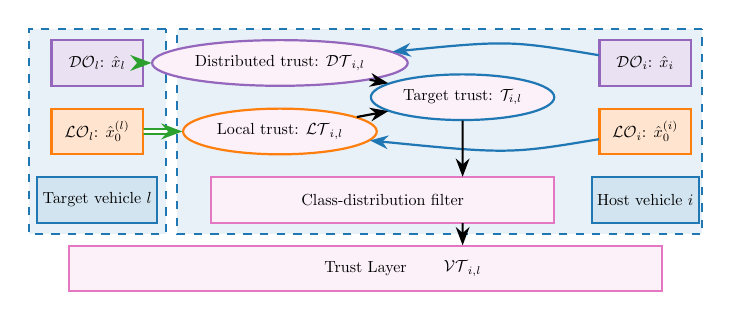
\begin{tikzpicture}[global scale = 0.58,
    vehicle/.style={draw=blue1, fill=blue1!20, thick, minimum width=2cm, minimum height=1cm},
    localobs/.style={draw=orange1, fill=orange1!20, thick, minimum width=2cm, minimum height=1cm},
    distobs/.style={draw=purple1, fill=purple1!20, thick, minimum width=2cm, minimum height=1cm},
    sigarrow/.style={-Stealth, thick, color=blue1},
    commarrow/.style={
    double,
    double distance=1pt,
    line width=0.7pt,
    draw=green1,
    -Stealth
    },
    physics/.style={draw=blue1, shape=rectangle, fill=blue1!10,line width=0.75pt,dashed,minimum width=3cm, minimum height=4.5cm}, %
    trustlayer/.style={draw=rose1, shape=rectangle, fill=rose1!10,thick,minimum width=13cm, minimum height=1cm},
    trust/.style={draw=rose1, shape=ellipse, fill=rose1!10,thick,minimum width=1.5cm, minimum height=1cm}
]

        \node[physics,line width=0.75pt,minimum width=3cm, minimum height=4.5cm] at(2,1.5) { };
        \node[vehicle, name=target] at(2,0) {Target vehicle $l$};
        \node[localobs, name=LOt] at(2,1.5) {$\LO_{l}$: $\hat{x}_{0}^{(l)}$};
        \node[distobs, name=DOt] at(2,3) {$\DO_{l}$: $\hat{x}_{l}$};

        \node[physics,line width=0.75pt,minimum width=11.5cm, minimum height=4.5cm,name=host] at(9.5,1.5) {};
        \node[vehicle,name=host] at(14,0) {Host vehicle $i$};
        \node[localobs,name=LOh] at(14,1.5) {$\LO_{i}$: $\hat{x}_{0}^{(i)}$};
        \node[distobs,name=DOh] at(14,3) {$\DO_{i}$: $\hat{x}_{i}$};

        \node[trust,draw = purple1, name=DT] at(6,3) {Distributed trust: $\DT_{i,l}$};
        \node[trust,draw = orange1, name=LT] at(6,1.5) {Local trust:  $\LT_{i,l}$};
        \node[trust,draw = blue1, name=T] at(10,2.25) {Target trust: $\T_{i,l}$};

        \node[trust,shape=rectangle,name=evo, minimum width=7.5cm] at(8.25,0) {Class-distribution filter};
        \node[name=evo,minimum height=1cm] at(10,0) {};

        \node[trustlayer] at(0.5/2+15.25/2,-1.5) {Trust Layer};
        \node[name = VT,minimum height=1cm] at(10,-1.5) {$\VT_{i,l}$};

        \draw[commarrow] (DOt) -- (DT);
        \draw[commarrow] (LOt) -- (LT);

        \draw[sigarrow] (LOh) .. controls +(-3,-0.5).. (LT);
        \draw[sigarrow] (DOh) .. controls +(-3,0.5).. (DT);

        \draw[sigarrow, black] (LT) -- (T);
        \draw[sigarrow,black] (DT) -- (T);

        \draw[sigarrow,black] (T) -- (evo);
        \draw[sigarrow,black] (evo) -- (VT);
    \end{tikzpicture}
    \caption{Trust framework.}
    \label{fig_trust_framework}
\end{figure}

In this context, we define the following types of trust:
\begin{itemize}
    \item \textbf{Local Trust $\LT_{i,l}$}: reliability of vehicle $l$'s local-observer data.
    \item \textbf{Distributed Trust $\DT_{i,l}$}: agreement between distributed estimates from $l$ and those of $i$.
    \item \textbf{Target Trust $\T_{i,l}$}: instantaneous fusion of Local Trust and Distributed Trust.
    \item \textbf{Vehicle Trust $\VT_{i,l}$}: class-filtered trust score used by the observer.
\end{itemize}

The following subsections define these scores and their use in the observer.
\subsection{Data validity indicator}

Before trust computation, each received V2V packet is checked for authenticity and freshness:
{\small
\begin{equation}
    \delta_{i,l}(t)=
    \begin{cases}
        1, & \text{if the message is authenticated and fresh}, \\
        0, & \text{otherwise.}
    \end{cases}
\end{equation}
}
Only packets with $\delta_{i,l}(t)=1$ are used for trust evaluation.

\subsection{Local trust}\label{sub:local_trust}

Local Trust $\LT_{i,l}$ measures the confidence of host vehicle $i$ in the local-observer output of neighbor $l \in \N_i$.
It uses bicycle-state consistency indicators: planar position, speed, heading, and an optional input-consistency check for acceleration and steering. Missing data are handled by a hold-and-decay rule.

\subsubsection{Planar position consistency}
Let $p_i=[X_i,Y_i]^\top$. The host transforms its onboard relative measurement of vehicle $l$ into the global frame and denotes it by $r_{i,l}^{\mathrm{meas}}(t)\in\mathbb{R}^2$. The relative position implied by the local observers is
\begin{equation*}
    r_{i,l}^{\mathrm{obs}}(t)=
    \begin{bmatrix}\hat X_0^{(l)}(t)-\hat X_0^{(i)}(t)\\
    \hat Y_0^{(l)}(t)-\hat Y_0^{(i)}(t)
    \end{bmatrix}.
\end{equation*}
The position-consistency score is
\begin{equation*}
    \iota_{i,l}^{\text{pos}}
    =
    \max\left(
    1 -
    \frac{\left\|r_{i,l}^{\mathrm{obs}}-r_{i,l}^{\mathrm{meas}}\right\|}
    {\varepsilon_p+\left\|r_{i,l}^{\mathrm{meas}}\right\|},
    0
    \right),
\end{equation*}
where $\varepsilon_p>0$ avoids division by zero.

\subsubsection{Speed consistency}
The host compares the relative speed implied by the two local observers with the onboard measured relative speed $v_{i,l}^{\mathrm{rel,meas}}(t)$:
\begin{equation*}
    \iota_{i,l}^{\text{speed}}
    =
    \max\left(
    1 -
    \frac{\left|(\hat{v}_{0}^{(l)}-\hat{v}_{0}^{(i)})-v_{i,l}^{\mathrm{rel,meas}}\right|}
    {\varepsilon_v+\left|v_{i,l}^{\mathrm{rel,meas}}\right|},
    0
    \right),
\end{equation*}
where $\varepsilon_v>0$ avoids division by zero.

\subsubsection{Heading consistency}
Heading is checked using the reported yaw and a motion-derived yaw estimate. From two consecutive accepted position reports from vehicle $l$,
\begin{equation*}
    \psi_{l}^{\mathrm{pos}}(t)=
    \mathrm{atan2}\big(\hat Y_0^{(l)}(t)-\hat Y_0^{(l)}(t-1),
    \hat X_0^{(l)}(t)-\hat X_0^{(l)}(t-1)\big).
\end{equation*}
If radar azimuth or LiDAR shape orientation is available, it can replace or complement $\psi_l^{\mathrm{pos}}(t)$. The heading score is
\begin{equation*}
    \iota_{i,l}^{\text{heading}} =
    \max\left(
    1-\frac{\left|\mathrm{wrap}_{\pi}(\hat{\psi}_0^{(l)}-\psi_l^{\mathrm{pos}})\right|}
    {\varepsilon_{\psi}+\psi_{\mathrm{th}}},
    0
    \right),
\end{equation*}
where $\psi_{\mathrm{th}}>0$ is a nominal heading tolerance. This check implements the heading-verification mechanism based on consecutive position reports or bearing measurements.
\begin{assumption}\label{assum_connect}
When a vehicle is connected, it has access to basic information about its neighbors, including their type, length, and nominal wheelbase class.
\end{assumption}

\subsubsection{Optional input consistency}
If acceleration and steering commands are included in the received packet, the host checks them against finite-difference speed and yaw-rate estimates:
\begin{align*}
    a_{l}^{\mathrm{fd}}(t)
    &=\frac{\hat v_0^{(l)}(t)-\hat v_0^{(l)}(t-n)}{nT_s},\\
    \omega_l^{\mathrm{bike}}(t)
    &=\frac{\hat v_0^{(l)}(t)}{L_w}\tan\hat\delta_l(t).
\end{align*}
With $\omega_l^{\mathrm{fd}}(t)=\mathrm{wrap}_{\pi}(\hat\psi_0^{(l)}(t)-\hat\psi_0^{(l)}(t-n))/(nT_s)$,
\begin{equation*}
    \iota_{i,l}^{\text{input}} =
    \max\left(
    1 -
    \frac{|\hat a_l-a_l^{\mathrm{fd}}|+|\omega_l^{\mathrm{bike}}-\omega_l^{\mathrm{fd}}|}
    {\varepsilon_u+a_{\mathrm{th}}+\omega_{\mathrm{th}}},
    0
    \right),
\end{equation*}
where $a_{\mathrm{th}}$ and $\omega_{\mathrm{th}}$ are nominal acceleration and yaw-rate tolerances. If the command channels are not transmitted, $\iota_{i,l}^{\text{input}}$ is omitted from the fusion.

\subsubsection{Fusion and update rule}
For simplicity and reproducibility, the available indicators are fused by multiplication. When the input channel is available, the local trust score is
\begin{equation}
    \LT_{i,l}^{\mathrm{raw}}(t)
    =\iota_{i,l}^{\text{pos}}(t)
    \iota_{i,l}^{\text{speed}}(t)
    \iota_{i,l}^{\text{heading}}(t)
    \iota_{i,l}^{\text{input}}(t).
    \label{eq_local_trust_product}
\end{equation}
If the optional input channel is unavailable, the last factor is omitted. Missing or invalid packets are handled by
\begin{equation}
    \LT_{i,l}(t) =
    \left\{ \begin{array}{lc}
        \LT_{i,l}^{\mathrm{raw}}(t),  &  \text{if } \delta_{i,l}(t) = 1, \\
        (1 - \lambda_h)\LT_{i,l}(t-1), & \text{otherwise}
    \end{array}\right.
    \label{eq_local_trust_update}
\end{equation}
where $\lambda_h$ sets the decay rate during data loss.
\begin{remark}
    Multiplicative fusion is conservative: one inconsistent channel is enough to reduce the local trust score. The decay $\lambda_h$ can increase with consecutive missed packets.
\end{remark}

\subsection{Distributed trust}
Distributed Trust applies the same idea to exchanged distributed estimates. It is defined as
\begin{equation}
        \DT_{i,l}(t)  = \begin{cases}
       \gamma_{i,l}^{\text{self}}(t) \cdot \gamma_{i,l}^{\text{local}}(t) \cdot
        \gamma_{i,l}^{\text{host}}(t)   &  \text{if } \delta_{i,l}(t) = 1 \\
        (1 - \lambda_h)\DT_{i,l}(t-1), & \text{otherwise} \\
    \end{cases}
\end{equation}
where $\gamma_{i,l}^{\text{self}}$, $\gamma_{i,l}^{\text{host}}$, and $\gamma_{i,l}^{\text{local}}$ check consistency with the sender's local observer, the host's distributed estimate, and the host's local measurements, respectively.

\subsubsection{Sender self-consistency}
The sender's distributed estimate of its own state should remain close to its local observer state:
\begin{equation}
    \begin{aligned}
    \gamma_{i,l}^{\text{self}}(t)
    &=
    \exp\Big(
    -(\hat{x}_l^{(l)}(t)\ominus\hat{x}_0^{(l)}(t))^{\top}
    \Sigma_{\text{self}}^{-1} \\
    &\qquad\quad \times
    (\hat{x}_l^{(l)}(t)\ominus\hat{x}_0^{(l)}(t))
    \Big),
    \end{aligned}
\end{equation}
where $\Sigma_{\text{self}}$ is the covariance matrix associated with the sender self-consistency residual.

\subsubsection{Host-estimate consistency}
The host compares the estimate received from target $l$ with its own estimate using the Mahalanobis distance:
\begin{equation}
    \rho_{i,l}^{(j)}(t) = \left( \hat{x}_i^{(j)}(t) \ominus \hat{x}_l^{(j)}(t) \right)^{\top} \Sigma_{\text{host}}^{-1} \left( \hat{x}_i^{(j)}(t) \ominus \hat{x}_l^{(j)}(t) \right)
    \label{eq_dis_glo}
\end{equation}
where $\Sigma_{\text{host}}$ is the diagonal covariance matrix of state-channel discrepancies:
\begin{equation}
\Sigma_{\text{host}} = \diag{\sigma^2_1, \sigma^2_2, \cdots , \sigma^2_n},
\end{equation}
where $n$ is the number of states and $\sigma^2_k$ is the variance of the $k$th state discrepancy.

The total discrepancy score is
\begin{equation}
    D_{i,l}^{\text{host}}(t) = \sum_{j=1}^N \rho_{i,l}^{(j)}(t).
\end{equation}
A small $D_{i,l}^{\text{host}}(t)$ means that vehicle $l$'s estimates are close to the host's estimates. The corresponding trust factor is
\begin{equation}
    \gamma_{i,l}^{\text{host}}(t) = \exp\left( -D_{i,l}^{\text{host}}(t) \right).
\end{equation}
where $\gamma_{i,l}^{\text{host}}(t) \in (0, 1]$.

\subsubsection{Consistency with host's local measurement}
Host vehicle $i$ uses relative measurements to nearby vehicles, e.g., planar relative position, range, bearing, relative speed, or heading difference, to check whether the estimates from target $l$ are consistent with local sensing.

Let $y_{i,j}(t) \in \mathbb{R}^{m_{ij}}$ be the relative measurement from vehicle $i$ to vehicle $j$, e.g., the global-frame relative position $p_j(t)-p_i(t)$ or a range-bearing vector transformed through the host pose.

The estimate received from target $l$ should approximately satisfy
\begin{equation*}
    H(\hat{x}_l^{(j)}(t) \ominus \hat{x}_l^{(i)}(t)) \approx y_{i,j}(t).
\end{equation*}
where $H \in \mathbb{R}^{m_{ij} \times n}$ extracts the measured states.

The consistency error is
\begin{equation}
    \varepsilon_{i,l}^{(j)}(t) = H\left( \hat{x}_l^{(j)}(t) \ominus \hat{x}_l^{(i)}(t) \right) - y_{i,j}(t),
\end{equation}
Using $\Sigma_{\text{local}}$ as in~\eqref{eq_dis_glo}, define
\begin{equation}
    E_{i,l}^{(j)}(t) = (\varepsilon_{i,l}^{(j)}(t))^{\top} \Sigma_{\text{local}}^{-1} \varepsilon_{i,l}^{(j)}(t).
\end{equation}

The total consistency error is
\begin{equation}
    E_{i,l}(t) = \sum_{j \in \N_i} E_{i,l}^{(j)}(t).
\end{equation}
A higher $E_{i,l}(t)$ means that the estimates from target $l$ disagree with local relative measurements.

The trust factor is
\begin{equation}
    \gamma_{i,l}^{\text{local}}(t) = \exp\left( -{E_{i,l}(t)} \right),
\end{equation}
where $\gamma_{i,l}^{\text{local}}(t) \in (0, 1]$.
\begin{remark}
The covariance matrices $\Sigma_{\text{host}}$ and $\Sigma_{\text{local}}$ can be estimated from a recent nominal-data window at vehicle \(i\), avoiding covariance transmission between nodes.
\end{remark}
\subsection{Target trust and temporal evolution}\label{subsec_evolution}
We combine the Local Trust and Distributed Trust into a single instantaneous trust score for target $l$:
\begin{equation}
    \T_{i,l}(t) =  \LT_{i,l}(t) \cdot \DT_{i,l}(t).
    \label{trs_sample_genral}
\end{equation}
$\T_{i,l}(t)$ measures the instantaneous quality of target $l$'s data.
Because this value can vary abruptly, a class-distribution temporal filter is used instead of applying the instantaneous scalar directly.
Let $q=5$ denote the number of ordered trust classes:
\textit{Unreliable}, \textit{Poor}, \textit{Acceptable}, \textit{Good}, and \textit{Excellent}.
Define the class scores
\begin{equation}
    \rho_m=\frac{m-1}{q-1}, \qquad m=1,\ldots,q,
\end{equation}
and the corresponding intervals
\begin{equation}
    \mathcal{I}_m =
    \begin{cases}
    \left[\dfrac{m-1}{q},\dfrac{m}{q}\right), & m=1,\ldots,q-1,\\[1ex]
    \left[\dfrac{q-1}{q},1\right], & m=q.
    \end{cases}
\end{equation}
The instantaneous trust value is discretized into a one-hot class vector
\begin{equation}
    r_{i,l,m}(t)=
    \begin{cases}
    1, & \T_{i,l}(t)\in \mathcal{I}_m,\\
    0, & \text{otherwise,}
    \end{cases}
    \qquad
    r_{i,l}(t)\in\mathbb{R}^{q}.
\end{equation}
For example, $\T_{i,l}(t)=0.72$ belongs to the \textit{Good} class for $q=5$, so $r_{i,l}(t)=[0,0,0,1,0]^\top$.

The accumulated class evidence is updated as
\begin{equation}
    R_{i,l}(t+1)=
    \left(1-\beta_{\text{trust}}\T_{i,l}(t)\right)R_{i,l}(t)
    +r_{i,l}(t),
    \label{eq_class_history_update}
\end{equation}
where $R_{i,l}(t)\in\mathbb{R}_{\ge0}^{q}$ is initialized as $R_{i,l}(0)=0$ unless prior interaction evidence is available, and $\beta_{\text{trust}}\in[0,1]$ controls the decay of past class evidence.
The modulation by $\T_{i,l}(t)$ prevents one isolated low-quality sample from immediately erasing the accumulated history, while repeated low-quality samples keep adding evidence to the lower classes.
To regularize the class distribution, let $\alpha_{\mathrm{tr}}\in\mathbb{R}_{\ge0}^{q}$ be a prior trust-class distribution satisfying $\sum_{m=1}^{q}\alpha_{\mathrm{tr},m}=1$, and let $C_{\mathrm{tr}}>0$ be a confidence parameter.
The prior $\alpha_{\mathrm{tr}}$ represents the initial belief about vehicle $l$ before enough packets are observed; if no prior information is available, one can use the uniform choice $\alpha_{\mathrm{tr},m}=1/q$.
The parameter $C_{\mathrm{tr}}$ controls how strongly this prior affects the estimate: larger $C_{\mathrm{tr}}$ gives more weight to the prior, while smaller $C_{\mathrm{tr}}$ lets online evidence dominate faster.
The normalized trust-class distribution is
\begin{equation}
    S_{i,l,m}(t)=
    \frac{R_{i,l,m}(t)+C_{\mathrm{tr}}\alpha_{\mathrm{tr},m}}
    {C_{\mathrm{tr}}+\sum_{s=1}^{q}R_{i,l,s}(t)},
    \qquad m=1,\ldots,q.
    \label{eq_class_distribution}
\end{equation}
The smoothed vehicle trust used by the observer is the expected trust level
\begin{equation}
    \VT_{i,l}(t)=
    \sum_{m=1}^{q}\rho_m S_{i,l,m}(t).
    \label{eq_class_filtered_vehicle_trust}
\end{equation}
A larger $\beta_{\text{trust}}$ gives a more reactive trust history, while a smaller value gives smoother trust evolution.
The confidence $C_{\mathrm{tr}}$ controls how strongly the prior influences the estimate when only a short interaction history is available.
The observer uses $\VT_{i,l}(t)$ to weigh information received from vehicle $l$.

For the controller interface, each host vehicle also forms an opinion vector
\begin{equation}
    \O_i(t)=[\O_i(1,t),\ldots,\O_i(N,t)],
\end{equation}
where $\O_i(i,t)=1$ and $\O_i(l,t)=\VT_{i,l}(t)$ for trusted neighbors. For non-neighboring vehicles, $\O_i(j,t)$ can be obtained from one-hop propagated opinions or assigned a conservative default when no credible propagated opinion is available. This vector is used only as a compact reliability summary for the controller blending factor in Section~\ref{sec_simulation}; the observer-weight design below uses the pairwise trust values directly.

\section{Trust-Based Observer Weight Design}\label{sec_weight_design}
The trust framework provides each vehicle with smoothed vehicle-trust scores $\VT_{i,l}(t)$ representing the reliability of information from other vehicles.
This section shows how these values are used to define adaptive observer weights $w_{il}^{(j)}(t)$ and establishes conditions for stability of the estimation error dynamics.

\subsection{Weight based on the trust}
Using the virtual graph $\bar{\G}^{(j)}$, each vehicle $i$ first selects the trusted neighbor sources at time $t$:
\begin{equation}
\mathcal{LN}^{(j)}_{i}(t)
= \Big\{\, l \in \N_i \;\big|\; \VT_{i,l}(t) \ge \theta_{\min} \Big\}.
\end{equation}
The selected trust scores are then used directly as reliability scores,
\begin{align}
s_{i,l}^{(j)}(t)
&=
\begin{cases}
\VT_{i,l}(t), & l\in\mathcal{LN}^{(j)}_{i}(t),\\
0, & \text{otherwise},
\end{cases}
\label{new_setneibor}\\
S_i^{(j)}(t)
&=\epsilon+\sum_{r\in\N_i}s_{i,r}^{(j)}(t),
\end{align}
where $\epsilon>0$ avoids division by zero. Let $\eta_0,\eta_N\in[0,1]$ denote the local-anchor and neighbor-consensus budgets, respectively, with
\begin{equation}
    \eta_0+\eta_N\le1 .
\end{equation}
The local-anchor weight is
\begin{equation}\label{eq_anchor_weight}
w_{i0}^{(j)}(t)=
\begin{cases}
\eta_0\LT_{i,j}(t), & \LT_{i,j}(t)\ge\theta_{\min},\\
0, & \text{otherwise},
\end{cases}
\end{equation}
and the neighbor weights are
\begin{equation}\label{design_gain}
    w_{il}^{(j)}(t)
    =
    \eta_N
    \frac{s_{i,l}^{(j)}(t)}
    {S_i^{(j)}(t)},
    \qquad l\in\N_i .
\end{equation}
Thus, rejected neighbors receive zero weight, while accepted neighbors share the fixed budget $\eta_N$ in proportion to their trust values. The remaining mass is the implicit self-prediction weight
\begin{equation}
    w_{is}^{(j)}(t)
    =
    1-w_{i0}^{(j)}(t)-\sum_{l\in\N_i}w_{il}^{(j)}(t).
\end{equation}
These weights induce a switching communication graph because the trusted-neighbor set changes online. We assume:
\begin{assumption}[\it Jointly connected graph]%\label{def1}
\label{ass_graph}
There exists a scalar constant $T > 0$ such that for all $t\geq 0$, the union graph $\bigcup_{\tau\in[t,\,t+T]}\bar{\G}^{(j)}(\tau)$ contains a spanning tree.
\end{assumption}
Assumption~\ref{ass_graph} means that every node $i \in\V$ is reachable from node ``0'' over each time window $[t,t+T]$, ensuring enough connectivity for the observer design~\cite{hao2024eventtriggered}.

\subsection{Stability of the error}\label{subsec_Prove}
We now state sufficient conditions for stability of the local time-varying error dynamics obtained by linearizing the bicycle model along bounded trajectories. Let $A_j(t)$, $B_j(t)$, and $C_j(t)$ denote the Jacobians of vehicle $j$ evaluated along the corresponding nominal or estimated trajectory, and absorb higher-order linearization remainders into the disturbance terms. The nominal errors satisfy
\begin{equation}\label{eq_e0}
   e_0^{(j)}(t+1) = \left( A_j(t) - F_{j}(t) C_j(t)  \right) e_0^{(j)}(t) + d_0^{(j)}(t),
\end{equation}
{\small
    \begin{align}\label{eq_error}
        e_{\DO}^{(j)}(t+1) &= \left( w_{0}^{(j)}(t) \otimes A_j(t) \right) e_0^{(j)}(t)  \notag\\
        &+ \left( \left( I_{N} - \bar{\L}^{(j)}(t)  \right)  \otimes  A_j(t) \right) e_{\DO}^{(j)}(t) + d_{\DO}^{(j)}(t),
    \end{align}
}
with
{\small
\begin{align*}
    \bar{\L}^{(j)}(t)&=\left[\bar{l}_{ik}^{(j)}(t)\right],
    \bar{l}_{ii}^{(j)}(t) =\sum_{l\in \N_i\cup\{0\}} w_{il}^{(j)}(t),\\
    \bar{l}_{ik}^{(j)}(t)&=
    \begin{cases}
    -w_{ik}^{(j)}(t), & k\neq i,\; k\in\N_i,\\
    0, & k\neq i,\; k\notin\N_i.
    \end{cases}
\end{align*}
}
\begin{align*}
    d_0^{(j)}(t) &= r_0^{(j)}(t)- \Delta_j(t), \\
    d_{\DO}^{(j)}(t)  &= (I_N \otimes B_j(t))(\hat{u}_j(t)-u_j(t)) \\
    &\quad + r_{\DO}^{(j)}(t) - (\mathbf{1}_N \otimes \Delta_j(t)), \\
    e_{\DO}^{(j)}(t) &= \col{e_1^{(j)}(t), \cdots , e_N^{(j)}(t)}
\end{align*}
where $r_0^{(j)}$ and $r_{\DO}^{(j)}$ collect bounded nonlinear linearization remainders, and
$w_{0}^{(j)}(t) = \col{w_{10}^{(j)}(t), \cdots, w_{N0}^{(j)}(t)} $ is a vector describing the connection between the local observer $(\LO_{j})$ and other distributed observers $(\DO_{i})$, $i \in \V$; $\bar{\L}^{(j)}(t)$ is the virtual weighted Laplacian matrix of the virtual graph $\bar{\G}^{(j)}(t)$.

The attack contribution can be written explicitly in the same error system.
Suppose that a received channel is corrupted before the correction step.
For compact notation, the receiving-host index is suppressed and host vehicle $i$ receives
\begin{equation}
    \tilde{x}_{0}^{(j)}(t)=\hat{x}_{0}^{(j)}(t)+a_{0}^{(j)}(t),
    \qquad
    \tilde{x}_{l}^{(j)}(t)=\hat{x}_{l}^{(j)}(t)+a_{l}^{(j)}(t),
\end{equation}
where $a_{0}^{(j)}$ corrupts the local-anchor signal and $a_{l}^{(j)}$ corrupts the distributed estimate received from neighbor $l$.
Let $\mathcal{M}_{i}^{(j)}(t)\subseteq\N_i$ denote the attacked neighbor channels at host $i$; for unattacked, unavailable, or rejected channels, the corresponding attack vector is set to zero.
Then host $i$ receives the additive attack input
{\small
\begin{equation}
d_{\mathrm{att},i}^{(j)}(t)
=A_j(t)\left(w_{i0}^{(j)}(t)a_{0}^{(j)}(t)+\sum_{l\in\mathcal{M}_{i}^{(j)}(t)}w_{il}^{(j)}(t)a_{l}^{(j)}(t)\right).
\label{eq_attack_input}
\end{equation}
}
Stacking the row-wise terms gives
\begin{equation}
    d_{\mathrm{att}}^{(j)}(t)
    =\col{d_{\mathrm{att},1}^{(j)}(t),\ldots,d_{\mathrm{att},N}^{(j)}(t)}.
\end{equation}
Substituting the corrupted signals into~\eqref{eq_DO}, the attacked observer has the same theorem form:
{\small
\begin{align}
e_{\DO}^{(j)}(t+1)
&= \left( w_{0}^{(j)}(t) \otimes A_j(t) \right) e_0^{(j)}(t)  \notag\\
&\quad+ \left( \left( I_{N} - \bar{\L}^{(j)}(t)  \right)  \otimes  A_j(t) \right) e_{\DO}^{(j)}(t)
+\tilde d_{\DO}^{(j)}(t),
\label{eq_error_attacked}
\end{align}
}
with
{\small
\begin{equation}
    \tilde d_{\DO}^{(j)}(t)
    =d_{\DO}^{(j)}(t)+d_{\mathrm{att}}^{(j)}(t).
\end{equation}
}
Thus, the attack does not change the homogeneous transition matrix of the distributed error; it adds an input whose size is modulated by the trust weights.
If $\|a_{0}^{(j)}(t)\|_*\le \bar a_0$ and $\|a_{l}^{(j)}(t)\|_*\le \bar a_{\mathrm{N}}$ on $\mathcal{M}_{i}^{(j)}(t)$, then Lemma~\ref{lem_weight_admissible} gives
\begin{align}
\|d_{\mathrm{att},i}^{(j)}(t)\|_*
&\le \|A_j(t)\|_*
\left(
w_{i0}^{(j)}(t)\bar a_0
+\sum_{l\in\mathcal{M}_{i}^{(j)}(t)}
w_{il}^{(j)}(t)\bar a_{\mathrm{N}}
\right) \notag\\
&\le \bar A_j \max\{\bar a_0,\bar a_{\mathrm{N}}\}.
\label{eq_attack_bound}
\end{align}
Because the bicycle trajectory and steering angle are assumed bounded away from the singular steering limit, there is a finite $\bar A_j$ satisfying $\|A_j(t)\|_*\le\bar A_j$. Consequently, for the stacked vector there exists a finite constant $\bar d_{\mathrm{att}}$ such that
\begin{equation}
    \|d_{\mathrm{att}}^{(j)}(t)\|\le \bar d_{\mathrm{att}}.
\end{equation}
When the trust layer rejects a corrupted channel, the associated weight becomes zero and its contribution in~\eqref{eq_attack_input} disappears.

We assume bounded disturbances and bounded additive attacks.
\begin{assumption}\label{assum_distur}
There exist $\bar{d}_{0} \geq 0$, $\bar{d}_{\DO} \geq 0$, and $\bar d_{\mathrm{att}}\ge0$ such that, for all $t\geq 0$,
\[
\|d_0^{(j)}(t)\| \le \bar{d}_{0},
\qquad
\|d_{\DO}^{(j)}(t)\| \le \bar{d}_{\DO},
\qquad
\|d_{\mathrm{att}}^{(j)}(t)\| \le \bar d_{\mathrm{att}}.
\]
Equivalently, the attacked distributed-error input satisfies
\[
    \|\tilde d_{\DO}^{(j)}(t)\|\le
    \bar{\tilde d}_{\DO}:=\bar d_{\DO}+\bar d_{\mathrm{att}}.
\]
\end{assumption}

\begin{lemma}[Local-observer ISS]\label{lem_local_iss}
If the time-varying local error transition $A_j(t)-F_j(t)C_j(t)$ is uniformly exponentially stable and Assumption~\ref{assum_distur} holds, then the local-observer error~\eqref{eq_e0} is ISS with respect to $d_0^{(j)}$. In particular, there exist $c_{\ell}>0$ and $\lambda_{\ell}\in(0,1)$ such that
\begin{equation}
\|e_0^{(j)}(t)\|\le c_{\ell}\lambda_{\ell}^{t}\|e_0^{(j)}(0)\|
+\frac{c_{\ell}}{1-\lambda_{\ell}}\bar d_0 .
\end{equation}
\end{lemma}
\begin{proof}
Let $\Phi_{\ell,j}(t,k)$ be the transition product of $A_j(\tau)-F_j(\tau)C_j(\tau)$ from $\tau=k$ to $t-1$. Uniform exponential stability gives constants $c_{\ell}>0$ and $\lambda_{\ell}\in(0,1)$ such that $\|\Phi_{\ell,j}(t,k)\|\le c_{\ell}\lambda_{\ell}^{t-k}$. Unrolling~\eqref{eq_e0} and using Assumption~\ref{assum_distur} gives the stated geometric bound.
\end{proof}

\begin{lemma}[Admissibility of trust weights]\label{lem_weight_admissible}
The weight law~\eqref{new_setneibor}--\eqref{design_gain} satisfies $w_{il}^{(j)}(t)\ge0$, $w_{i0}^{(j)}(t)\ge0$, and
\begin{equation}
\sum_{l\in\N_i\cup\{0\}}w_{il}^{(j)}(t)\le1
\end{equation}
for all $i,j$ and all $t$.
\end{lemma}
\begin{proof}
By construction, $s_{i,l}^{(j)}(t)\ge0$ and $S_i^{(j)}(t)>0$, hence $w_{il}^{(j)}(t)\ge0$ for all $l\in\N_i$. Also, $0\le w_{i0}^{(j)}(t)\le \eta_0$ because $\LT_{i,j}(t)\in[0,1]$. The neighbor contribution satisfies
\begin{align*}
\sum_{l\in\N_i}w_{il}^{(j)}(t)
&=
\eta_N
\frac{\sum_{l\in\N_i}s_{i,l}^{(j)}(t)}
{\epsilon+\sum_{l\in\N_i}s_{i,l}^{(j)}(t)}
\le \eta_N .
\end{align*}
Therefore,
\[
\sum_{l\in\N_i\cup\{0\}}w_{il}^{(j)}(t)
=w_{i0}^{(j)}(t)+\sum_{l\in\N_i}w_{il}^{(j)}(t)
\le \eta_0+\eta_N\le1 .
\]
\end{proof}

\begin{lemma}[Distributed-error contraction]\label{lem_dist_contraction}
Suppose that condition~\eqref{assume3} holds. If the local-observer error is ISS and Assumption~\ref{assum_distur} holds, then the nominal distributed error~\eqref{eq_error} is ISS with respect to $e_0^{(j)}$ and $d_{\DO}^{(j)}$. Under the additive attack model~\eqref{eq_error_attacked}, the attacked distributed error is ISS with respect to $e_0^{(j)}$ and $\tilde d_{\DO}^{(j)}$.
\end{lemma}
\begin{proof}
Let $\Phi_{\DO}^{(j)}(t)=((I_N-\bar{\L}^{(j)}(t))\otimes A_j(t))$.
Under~\eqref{assume3}, $\|\Phi_{\DO}^{(j)}(t)\|_*\le\alpha<1$ uniformly over all admissible trust-induced switches and all bounded bicycle trajectories considered. Iterating~\eqref{eq_error} yields a sum of products of $\Phi_{\DO}^{(j)}(\cdot)$ multiplying the initial error, the local-anchor input $(w_0^{(j)}\otimes A_j)e_0^{(j)}$, and $d_{\DO}^{(j)}$. The products are bounded by powers of $\alpha$, while Lemma~\ref{lem_local_iss} and Assumption~\ref{assum_distur} bound the two inputs. The resulting geometric series gives an ISS bound.
For~\eqref{eq_error_attacked}, the same iteration is obtained after replacing $d_{\DO}^{(j)}$ by $\tilde d_{\DO}^{(j)}=d_{\DO}^{(j)}+d_{\mathrm{att}}^{(j)}$. Since Assumption~\ref{assum_distur} gives $\|\tilde d_{\DO}^{(j)}(t)\|\le\bar{\tilde d}_{\DO}$, the attack contributes only an additional bounded input term and does not affect the contraction factor $\alpha$.
\end{proof}

The main ISS result is stated as follows.
\begin{theorem}\label{thm_observer}
Consider a vehicle platoon~\eqref{eq_platoon} over a directed weighted communication network $\bar{\G}^{(j)}$. Let~\eqref{eq_observer} be the corresponding distributed observer. Assume that the following conditions hold true:
\begin{enumerate}
    \item For all $j \in \V$, there exists a bounded gain $F_{j}(t)$ such that the time-varying matrix $A_j(t)-F_j(t)C_j(t)$ is uniformly exponentially stable along the considered bounded bicycle trajectory.
    \item For all $i \in \V$, $w_{i0}^{(j)} \geq 0$ and $w_{il}^{(j)} \geq 0$ satisfy
    \begin{equation}\label{thm_W}%\label{sum_w_il}
    \sum_{l\in \N_i\cup\{0\}} w_{il}^{(j)}(t) \leq 1.
    \end{equation}
    \item There exists $\alpha \in (0,1)$ and a matrix norm $\| \cdot \|_*$ such that, uniformly over all admissible switches,
	\begin{equation} \label{assume3}
        \| \left( I_{N} - \bar{\L}^{(j)}(t) \right)  \otimes  A_j(t) \|_* \leq \alpha < 1.
	\end{equation}
\end{enumerate}
Then, the estimation error~\eqref{eq_e0}--\eqref{eq_error} is ISS. Under the additive attack model~\eqref{eq_error_attacked}, the attacked estimation error is also ISS. In particular, there exist constants $c_0, c_1 > 0$ and $\lambda \in (0,1)$ such that
\begin{align}
\|e_0^{(j)}(t)\| &\le \lambda^t \|e_0^{(j)}(0)\| + c_0 \bar{d}_0,\\
\|e_{\DO}^{(j)}(t)\| &\le \lambda^t \|e_{\DO}^{(j)}(0)\| \notag\\
&\quad+ c_1 \Big(\|e_0^{(j)}(0)\| + \bar{d}_0 + \bar{\tilde d}_{\DO}\Big).
\end{align}

\end{theorem}
\begin{proof}
Condition~1 and Assumption~\ref{assum_distur} give the local-observer bound by Lemma~\ref{lem_local_iss}. Condition~2 is satisfied by the proposed trust-weight law according to Lemma~\ref{lem_weight_admissible}, and it also prevents a row of the trust-weighted mixing matrix from amplifying all incoming corrections beyond unit mass.
Define
\begin{align*}
    B_0^{(j)}(t)&=w_0^{(j)}(t)\otimes A_j(t),\\
    A_{\DO}^{(j)}(t)&=\left( I_N-\bar{\L}^{(j)}(t)\right)\otimes A_j(t) .
\end{align*}
Condition~3 gives $\|A_{\DO}^{(j)}(t)\|_*\le\alpha<1$ uniformly over the trust-induced switches.
For $0\le k<t$, let $\Psi(t,k)$ be the product of the matrices $A_{\DO}^{(j)}(\cdot)$ from time $k$ to time $t-1$. Then $\|\Psi(t,k)\|_*\le\alpha^{t-k}$, and the attacked recursion~\eqref{eq_error_attacked} gives
\begin{align*}
\|e_{\DO}^{(j)}(t)\|_*
&\le \alpha^t\|e_{\DO}^{(j)}(0)\|_*\\
&\quad+\sum_{k=0}^{t-1}\alpha^{t-1-k}
\|B_0^{(j)}(k)\|_*\|e_0^{(j)}(k)\|_*\\
&\quad+\sum_{k=0}^{t-1}\alpha^{t-1-k}
\|\tilde d_{\DO}^{(j)}(k)\|_* .
\end{align*}
The weights are bounded by Condition~2, so $\|B_0^{(j)}(k)\|_*\le\bar B_0$ for some finite $\bar B_0$. Lemma~\ref{lem_local_iss} bounds $e_0^{(j)}(k)$, and Assumption~\ref{assum_distur} bounds $\tilde d_{\DO}^{(j)}(k)$. The remaining sums are geometric; taking $\lambda=\max\{\alpha,\lambda_{\ell}\}$ and absorbing norm-equivalence constants and bounded input gains into $c_0$ and $c_1$ gives the stated ISS inequalities. In the nominal case, $d_{\mathrm{att}}^{(j)}=0$ and $\bar{\tilde d}_{\DO}=\bar d_{\DO}$.
\end{proof}

\begin{remark}
The conditions of Theorem~\ref{thm_observer} can be checked with standard Lyapunov arguments for the local linearized bicycle model. The result is local in the usual nonlinear-observer sense: the trajectory, speed, steering angle, input mismatch, and linearization remainders must remain bounded in the operating region. The cascade structure allows the local error~\eqref{eq_e0} and distributed error~\eqref{eq_error} to be analyzed separately. The additive attack term in~\eqref{eq_attack_input} is therefore handled as an ISS input: bounded attacks produce bounded estimation degradation, and trust rejection reduces the corresponding input gain by driving the malicious weights to zero.
\end{remark}

\section{Contamination Rollback Under Delayed Trust Decisions}\label{sec_rollback}
Trust values are computed from consistency windows and therefore may lag behind the first corrupted packet. During this detection delay, falsified data can enter the distributed observer before the corresponding neighbor is removed from the trusted set. To limit this transient contamination, each host vehicle can optionally maintain a finite rollback buffer and re-evaluate the most recent observer steps once a neighbor is flagged.

The rollback module is useful when contamination is propagated through an otherwise honest intermediate vehicle. Consider an attacked transmitter $l^{\star}$ and two honest vehicles $m$ and $i$. During the trust-detection delay, $l^{\star}$ broadcasts a falsified position or heading, and vehicle $m$ uses this packet in its own distributed estimate before the trust score has fallen below the rejection threshold. Later, vehicle $i$ receives the fleet estimate from $m$. From the direct perspective of vehicle $i$, the neighbor $m$ may still appear reliable, but the estimate carried by $m$ already contains upstream contamination from $l^{\star}$. If the observer only sets future weights associated with $l^{\star}$ to zero after detection, the biased state that entered the recursion during the previous steps remains embedded in the current estimate and can continue to affect prediction. Rollback is introduced to address exactly this delayed-decision effect: when the unreliable source is identified, the host returns to a recent stored state, removes the newly rejected contribution from the buffered updates, and replays the observer with the local anchor and the remaining trusted neighbors. Thus, rollback converts a late trust decision into a retrospective correction rather than only a future communication cut.

Assume that neighbor $l^{\star}$ is declared unreliable at time $t$. For a rollback horizon $K$, host vehicle $i$ stores, for each observer $\DO_i^{(j)}$ and each time $k\in\{t-K,\ldots,t-1\}$, the pre-update state $\hat{x}_i^{(j)}(k)$, the received neighbor estimates, the trust weights, the anchor estimate, and the input estimate $\hat{u}_j(k)$. During replay, the corrected state $x_{\mathrm{r}}$ is used to recompute the innovation terms
\begin{align}
\tilde{\eta}_{il}^{(j)}(k;x_{\mathrm{r}})
&= w_{il}^{(j)}(k)
\big(\hat{x}_l^{(j)}(k)\ominus x_{\mathrm{r}}\big),\quad l\in\N_i, \\
\tilde{\eta}_{i0}^{(j)}(k;x_{\mathrm{r}})
&= w_{i0}^{(j)}(k)
\big(\hat{x}_0^{(j)}(k)\ominus x_{\mathrm{r}}\big).
\end{align}
When $l^{\star}$ is flagged, the host resets the temporary state to the buffer start,
\begin{equation}
    x_{\mathrm{r}} \leftarrow \hat{x}_i^{(j)}(t-K),
\end{equation}
and replays the observer update for $k=t-K,\ldots,t-1$ while excluding the flagged neighbor, or a flagged set $\mathcal{M}$:
\begin{equation}
\begin{aligned}
x_{\mathrm{r}} \leftarrow\;&
f_{\text{b}}\!\left(
x_{\mathrm{r}}
+\sum_{l\in\N_i\setminus\mathcal{M}}\tilde{\eta}_{il}^{(j)}(k;x_{\mathrm{r}})
+ \tilde{\eta}_{i0}^{(j)}(k;x_{\mathrm{r}}),
\hat{u}_j(k)\right).
\end{aligned}
\label{eq_rollback_replay}
\end{equation}
Finally, the current distributed estimate is corrected by setting
\begin{equation}
    \hat{x}_i^{(j)}(t)\leftarrow x_{\mathrm{r}}.
\end{equation}
The rollback memory cost is proportional to $K\deg(i)$ per observer and can be implemented with archived packets and weights. The anchor innovation $\tilde{\eta}_{i0}^{(j)}(k;x_{\mathrm{r}})$ is retained during replay so that removing a corrupted neighbor does not leave the correction step purely open loop. For the ISS interpretation, the reset map is treated as an additional bounded jump in the observer state. A finite buffer and a dwell-time condition on successive trust-triggered resets prevent arbitrarily fast reset accumulation and preserve the boundedness guarantees of Theorem~\ref{thm_observer}.

\section{Simulation and Platform Results}\label{sec_simulation}

This section evaluates estimation accuracy, trust evolution, rollback behavior, platform deployment flow, and closed-loop platoon-control relevance under falsified, faulty, replay/delay, and DoS communication attacks on the kinematic bicycle state and input channels. The validation is organized around three questions: whether the trust layer detects unreliable data, whether the adaptive observer limits estimation error relative to non-trust baselines, and whether the resulting estimates remain useful for longitudinal platoon control after projection onto the road direction.

\subsection{Simulation setup}

The simulation uses four vehicles with all-to-all V2V communication. The observer runs onboard each vehicle, and small modeling variations are treated as uncertainties. The main parameters are $N=4$, $T_s=0.1$~s, wheelbase $L_w=2.8$~m, local-trust weights $(w_p,w_v,w_\psi,w_u)=(1.4,1.0,1.2,0.8)$, class-filter decay $\beta_{\text{trust}}=0.5$, class confidence $C_{\mathrm{tr}}=0.2$, $q=5$ trust classes, heading tolerance $\psi_{\mathrm{th}}=0.15$~rad, and $\theta_{\min}=0.5$.

\subsection{QCar/LIMO Platform Implementation}\label{sec:qcar_limo_platform}

The proposed observer is also implemented for a mixed QCar/LIMO small-scale vehicle platform, where each vehicle runs the same onboard estimation and communication stack. This implementation checks whether the trust-aware observer can operate with real sensor timing, packet exchange, and controller execution rather than only with offline simulation data. Each vehicle broadcasts its local state estimate, fleet estimate, trust summary, and packet status through the V2V layer. The receiving host stores these packets, evaluates physical and temporal consistency, updates the trust weights, and then runs the distributed observer with the local observer as an anchor.

Figure~\ref{fig:qcar_limo_scheme} summarizes the experimental flow. The host vehicle stack contains the sensor interface, local observer, vehicle logic, and control loop. Peer vehicles run the same stack and exchange UDP packets containing local estimates and trust reports. The trust-based observer converts consistency checks into adaptive fusion weights and produces a resilient fleet-state estimate for visualization, validation, and controller use. The attack channel can inject corrupted, delayed, or replayed packets so that the no-rollback and rollback cases can be compared under the same vehicle trajectory and communication structure.

\begin{figure*}[!t]
    \centering
    \includegraphics[width=\textwidth]{img/global_system_scheme_ieee_simple.png}
    \caption{QCar/LIMO experimental scheme for trust-aware cooperative state estimation. Each vehicle runs a local observer and vehicle-logic loop, exchanges V2V estimates and trust reports, and computes trust-weighted distributed estimates with optional rollback.}
    \label{fig:qcar_limo_scheme}
\end{figure*}

At the vehicle level, the controller separates longitudinal and lateral behavior. Longitudinal commands update the forward speed, while the lateral controller generates the yaw command used by the planar vehicle dynamics. The QCar and LIMO vehicles are therefore connected to the same normalized state interface, so the mixed platform can report position, velocity, yaw, trust score, and rollback-correction histories using the observer variables of this paper.

\begin{figure}[!t]
    \centering
    \includegraphics[width=\linewidth]{img/2system.png}
    \caption{Vehicle-level control and dynamics structure used for the QCar/LIMO experiment.}
    \label{fig:qcar_limo_vehicle_structure}
\end{figure}

The platform comparison is organized into two matched test cases. In the first case, the trust-aware observer runs without rollback, so packets accepted during the detection delay can temporarily contaminate the distributed estimate. In the second case, the same attack timing is repeated with the finite-window rollback enabled; when the delayed trust decision identifies the corrupted source, the host replays the recent observer window using the corrected trusted-neighbor set. The corresponding result panels are discussed in the Results subsection.

To make the platform results easier to inspect and reproduce, the QCar/LIMO source code and experimental resources used in this study are openly available at \url{https://github.com/kslhuy/QCar2_Cran}. An accompanying rollback-estimation demonstration video is provided at \url{https://youtu.be/t6-soznp6ks}.

\subsection{Baselines and Evaluation Metrics}
To make the contribution identifiable, the validation is organized around the configurations in Table~\ref{tab:baseline_matrix}. These baselines separate the value of trust weighting, local-observer anchoring, rollback, and closed-loop fallback.

\begin{table*}[!t]
\centering
\caption{Baseline configurations for validation.}
\label{tab:baseline_matrix}
\scriptsize
\begin{tabular}{p{3.2cm}ccccp{5.2cm}}
\toprule
\textbf{Configuration} & \textbf{Neighbor trust} & \textbf{Anchor} & \textbf{Rollback} & \textbf{Trust control} & \textbf{Purpose} \\
\midrule
Fixed-weight distributed observer & No & Yes & No & No & Shows the effect of fixed consensus weights under corrupted V2V data. \\
Local-only fallback & No & No & No & No & Gives the conservative performance when cooperation is completely disabled. \\
Trust-aware without anchor & Yes & No & No & Optional & Isolates the contribution of local-observer anchoring. \\
Trust-aware without rollback & Yes & Yes & No & Yes & Measures the baseline trust response before delayed-decision replay. \\
Proposed full method & Yes & Yes & Yes & Yes & Combines trust weights, anchor correction, optional rollback, and trust-modulated control. \\
\bottomrule
\end{tabular}
\end{table*}

The estimation metrics are root-mean-square error (RMSE), peak error, trust detection delay, recovery time, and false-positive trust drops. For a state channel $q\in\{X,Y,\psi,v\}$ and vehicle $i$, the RMSE over a horizon $\mathcal{T}$ is
\begin{equation}
\operatorname{RMSE}_{q,i}=
\sqrt{\frac{1}{|\mathcal{T}|}\sum_{t\in\mathcal{T}}
\left(q_i(t)-\hat q_i(t)\right)^2}.
\end{equation}
For the yaw channel, $q_i-\hat q_i$ is interpreted as $\mathrm{wrap}_{\pi}(\psi_i-\hat\psi_i)$. Recovery time is measured from the attack end time to the first time at which the estimation error remains below a nominal tolerance for the rest of the recovery window. The present closed-loop check focuses on whether the inter-vehicle spacing remains positive during the attack interval. A deeper closed-loop study can add spacing RMSE, lateral deviation, heading error, maximum acceleration, maximum jerk, and string amplification. Table~\ref{tab:metric_matrix} summarizes these evaluation metrics.

\begin{table*}[!t]
\centering
\caption{Quantitative metrics for estimation and closed-loop validation.}
\label{tab:metric_matrix}
\scriptsize
\begin{tabular}{p{3.0cm}p{4.3cm}p{6.1cm}}
\toprule
\textbf{Metric} & \textbf{Definition} & \textbf{Purpose} \\
\midrule
RMSE and peak error & Channel-wise estimation error for $X$, $Y$, $\psi$, and $v$ & Does the observer reduce attack-induced estimation degradation? \\
Detection delay & Time between attack onset and $\VT_{i,l}<\theta_{\min}$ & Does trust react quickly enough for control use? \\
Recovery time & Time after attack end until error returns to nominal band & Does the observer recover after data become reliable again? \\
False-positive trust drop & Fraction of benign time with $\VT_{i,l}<\theta_{\min}$ & Does the trust layer avoid unnecessary communication removal? \\
Minimum spacing & $\min_t((p_{i-1}(t)-p_i(t))^\top e_{\parallel}(t)-L)$ & Is the platoon collision-free under attack? \\
Lateral and heading error & $\max_t |(p_i(t)-p_i^{\mathrm{ref}}(t))^\top e_{\perp}(t)|$ and $\max_t|\mathrm{wrap}_{\pi}(\psi_i-\psi_i^{\mathrm{ref}})|$ & Does the bicycle estimate remain aligned with the lane or path? \\
Acceleration and jerk & $\max_t |u_i(t)|$ and $\max_t |u_i(t)-u_i(t-1)|/T_s$ & Are controller commands physically smooth? \\
String amplification & Ratio of downstream to upstream spacing/velocity peaks & Quantifies disturbance propagation in an extended closed-loop study. \\
\bottomrule
\end{tabular}
\end{table*}

Additional validation beyond the present four-vehicle all-to-all case can include sparse-topology tests, coordinated attacks from two vehicles, delayed trust decisions with rollback, and Monte Carlo runs with sensor noise, packet loss, and model mismatch. Sensitivity can be evaluated over $\theta_{\min}$, $\beta_{\text{trust}}$, rollback horizon $K$, and platoon sizes $N\in\{4,8,12\}$.

\subsection{Attack scenarios}\label{sec:attack_scenarios}
Six attacks on the leader data are considered, as summarized in Table~\ref{tab:attack_mix}. Each attack is broadcast to all followers during $[10, 15]$~s, and $p$ denotes the attack or fault occurrence probability.

\begin{table}[!ht]
\centering
\caption{Six bicycle-state attack cases in the scenario.}
\label{tab:attack_mix}
\scriptsize
\begin{tabular}{p{0.7cm}p{1.35cm}p{2.0cm}p{3.0cm}}
\toprule
\textbf{Case} & \textbf{Type} & \textbf{Target} & \textbf{Parameters} \\
\midrule
1 & Bias & Planar position $(X,Y)$ & bias = $[-5,\,1]^\top$~m \\
2 & Faulty & Planar position $(X,Y)$ & int. = 10~m, $p = 0.3$ \\
3 & Bias & Speed $v$ & bias = $-2$~m/s \\
4 & Bias/faulty & Heading $\psi$ & bias = $0.25$~rad, $p = 0.3$ \\
5 & Faulty & Input $(a,\delta)$ & int. = $(1.0~\mathrm{m/s^2},0.08~\mathrm{rad})$, $p = 0.3$ \\
6 & Drop & All bicycle-state packets & $p_\text{drop} = 0.5$ \\
\bottomrule
\end{tabular}
\end{table}

\begin{table}[!ht]
\centering
\caption{Extended validation scenarios.}
\label{tab:extended_scenarios}
\scriptsize
\begin{tabular}{p{1.4cm}p{2.1cm}p{3.2cm}}
\toprule
\textbf{Scenario} & \textbf{Variation} & \textbf{Purpose} \\
\midrule
S1 & Six attacks in Table~\ref{tab:attack_mix} & Single-source attack isolation. \\
S2 & Replay/delay with delayed flag & Rollback benefit and recovery time. \\
S3 & Two attacked vehicles & Coordinated corruption robustness. \\
S4 & Sparse predecessor graph & Connectivity dependence. \\
S5 & Monte Carlo noise/dropout & False-positive and average-case behavior. \\
S6 & $N=4,8,12$ & Scalability and string amplification. \\
\bottomrule
\end{tabular}
\end{table}

\subsection{Results}

Figure~\ref{fig:hybrid_heatmap} reports the normalized impact score, defined as the raw combined estimation error over $X$, $Y$, $\psi$, and $v$ divided by the maximum error over all vehicles and attacks. The DoS attack (Case~6) gives the largest impact score (0.872), while the speed-bias attack (Case~3) gives the smallest one (0.240). Among the vehicles, V4 is the most affected and V2 is the most resilient, with the lowest average impact score (0.362).
\begin{figure}[!ht]
    \centering
    
\includegraphics[width=0.8\linewidth]{fig/hybrid.jpg}
    \caption{Heatmap of normalized impact scores for all vehicles and bicycle-state attack cases.}
    \label{fig:hybrid_heatmap}
\end{figure}

\begin{figure}[!ht]
    \centering
    
\includegraphics[width=0.85 \linewidth]{fig/trust_all_new_huy.jpg}
    \caption{Trust score evolution during DoS attack ({\it\textbf{Case~6}}).}
    \label{fig:trust_Dos}
\end{figure}

Figure~\ref{fig:trust_Dos} shows the trust evolution for the DoS case. During $[10, 15]$~s, the trust scores of V2, V3, and V4 drop below the threshold $\theta_{\min}=0.5$ and recover after the attack ends, showing that the proposed mechanism detects and isolates unreliable data online.

For the closed-loop controller, the present validation is limited to the attack window $[10,15]$~s. In this interval, the projected inter-vehicle spacing remains positive while the cooperative command is attenuated by the trust factor when unreliable packets are detected. Therefore, the current controller evidence supports spacing preservation during the tested attack interval; full string-stability analysis is left to the extended validation in Table~\ref{tab:extended_scenarios}.

\subsection{Distributed State Estimation for Platoon Control}
This subsection evaluates how the proposed bicycle-state estimates are used by the longitudinal platoon controller. The controller uses a road-aligned projection of the 2D state, so the observer remains two-dimensional while the spacing controller keeps the existing IDM/CACC structure. To avoid ambiguity, the controller does not mix local and distributed states directly. Instead, it computes two acceleration commands: a local IDM command driven by onboard information and a cooperative CACC command driven by the distributed observer. The final acceleration is obtained by trust-based command fusion. Steering or path-following control can be handled by a separate lane-tracking module using the estimated $(Y,\psi)$ channels.

\subsubsection{Notation}
For each host vehicle $i$, the local observer state
\begin{equation}
    \hat{x}_0^{(i)}=[\hat X_0^{(i)},\hat Y_0^{(i)},\hat\psi_0^{(i)},\hat v_0^{(i)}]^\top
\end{equation}
is the ego estimate produced from onboard sensing and the local model. The distributed estimate of vehicle $j$ computed onboard vehicle $i$ is
\begin{equation}
    \hat{x}_i^{(j)}=[\hat X_i^{(j)},\hat Y_i^{(j)},\hat\psi_i^{(j)},\hat v_i^{(j)}]^\top .
\end{equation}
The stack $\hat{x}_i=\col{\hat{x}_i^{(1)},\ldots,\hat{x}_i^{(N)}}$ is sometimes called a global estimate because it contains the platoon state, but it remains fully distributed: each host keeps its own copy. Let $\mathcal{P}_i=\{1,\ldots,i-1\}$ denote the preceding vehicles used by the cooperative layer. Let $e_{\parallel}(t)=[\cos\psi_{\mathrm{ref}}(t),\sin\psi_{\mathrm{ref}}(t)]^\top$ be the local road tangent and define the longitudinal coordinate $s_i(t)=p_i(t)^\top e_{\parallel}(t)$ with $p_i=[X_i,Y_i]^\top$.
For estimates, $\hat p_0^{(i)}=[\hat X_0^{(i)},\hat Y_0^{(i)}]^\top$ and $\hat p_i^{(j)}=[\hat X_i^{(j)},\hat Y_i^{(j)}]^\top$.

\subsubsection{Inner/Local Controller: Intelligent Driver Model}
The local controller uses only $\hat{x}_0^{(i)}$ and onboard relative sensing to the immediate predecessor. Its acceleration command is
\begin{align}
    u_{\mathrm{loc},i}
    &\equiv a_{\text{IDM},i} \notag\\
    &=\alpha\Bigg[
    1-\left(\frac{\hat{v}_0^{(i)}}{v_0}\right)^{\delta_{\mathrm{IDM}}}
    -\left(\frac{s^*(\hat{v}_0^{(i)},\Delta v_{i-1,i})}{s_{i-1,i}}\right)^2
    \Bigg],
\end{align}
where $s_{i-1,i}=(p_{i-1}-p_i)^\top e_{\parallel}-L$, $\Delta v_{i-1,i}=v_{i-1}-\hat{v}_0^{(i)}$, and
\begin{equation}
    s^*(\hat{v}_0^{(i)},\Delta v_{i-1,i})=s_0+T\hat{v}_0^{(i)}+\frac{\hat{v}_0^{(i)}\Delta v_{i-1,i}}{2\sqrt{\alpha\beta}}.
\end{equation}
Here $\alpha$, $\beta$, $\delta_{\mathrm{IDM}}$, $v_0$, $s_0$, and $T$ are the maximum acceleration, comfortable deceleration, free-flow exponent, desired velocity, minimum spacing, and time headway, respectively. Since $u_{\mathrm{loc},i}$ does not use V2V packets, it provides the safety fallback when the distributed layer is down-weighted.

\subsubsection{Cooperative Controller: Cooperative Adaptive Cruise Control}
The cooperative controller uses the distributed observer estimates of preceding vehicles together with the host's local ego estimate. Its command is
\begin{align}
    u_{\mathrm{coop},i}
    &\equiv u_{\text{CACC},i}(k) \notag\\
    &= \sum_{j\in\mathcal{P}_i} \Big[
    \kappa_s e_{s,ij}(k)
    + \kappa_v e_{v,ij}(k)
    + \kappa_{\psi} e_{\psi,ij}(k)\Big],
\end{align}
where
\begin{align*}
    e_{s,ij}(k)&=\big(\hat p_i^{(j)}(k)-\hat p_0^{(i)}(k)\big)^\top e_{\parallel}(k)-d_{i,j}(k),\\
    e_{v,ij}(k)&=\hat{v}_i^{(j)}(k)-\hat{v}_0^{(i)}(k),\\
    e_{\psi,ij}(k)&=\mathrm{wrap}_{\pi}\big(\hat\psi_i^{(j)}(k)-\hat\psi_0^{(i)}(k)\big).
\end{align*}
Here $d_{i,j}(k)$ is the CTHS distance from vehicle $i$ to predecessor $j$; for a homogeneous platoon it can be chosen as $d_{i,j}(k)=(i-j)(d+h\hat{v}_0^{(i)}(k))$. The gains $\kappa_s$, $\kappa_v$, and $\kappa_{\psi}$ weight projected position, speed, and heading-alignment errors. Thus, unreliable distributed estimates affect only $u_{\mathrm{coop},i}$ and are attenuated by the trust fusion below.

\subsubsection{Trust-Based Controller Fusion}
The final target acceleration blends the local and cooperative commands as
\begin{equation}
    a_{\text{target},i}=(1-\gamma_i(t))u_{\mathrm{loc},i}+\gamma_i(t)u_{\mathrm{coop},i},
\end{equation}
where $\gamma_i(t)\in[0,1]$ is selected from the opinion vector defined in Section~\ref{sec_trust_score}. In the current controller version,
\begin{equation}
    \gamma_i(t)=\min_{j\in\mathcal{P}_i}\O_i(j,t).
\end{equation}
This conservative choice makes the cooperative channel small if any predecessor used by the CACC layer has low opinion. A first-order filter then smooths transitions between the two command sources:
\begin{equation}
    u_i(t)=u_i(t-1)+\tau_f\big(a_{\text{target},i}-u_i(t-1)\big),
\end{equation}
where $\tau_f$ is the filter time constant.

\subsubsection{Expected Distance}
For validation, the steady-state IDM spacing under $a_{\text{IDM},i}=0$ and $\Delta v_{i-1,i}=0$ is
\begin{equation}
    s_{i-1,i}=\frac{s_0+T\hat{v}_0^{(i)}}{\sqrt{1-\left(\dfrac{\hat{v}_0^{(i)}}{v_0}\right)^{\delta_{\mathrm{IDM}}}}}.
\end{equation}
For the CTHS policy, when the platoon reaches consensus, the spacing reference used by the current controller is
\begin{equation}
    s_{i-1,i}^{\mathrm{ref}}=d+h\hat{v}_0^{(i)}.
\end{equation}
The trust-modulated blending and the first-order filter are used to limit abrupt command changes when cooperative information is down-weighted.

\section{Discussion and Limitations}\label{sec_discussion}
The proposed method is designed to protect the platoon estimate and controller from unreliable incoming data, not to perform forensic reconstruction of a compromised vehicle. Once a neighbor is rejected by the trust layer, its information is no longer used as a cooperative correction source; accurate reconstruction of that vehicle then requires either a trusted independent measurement, a reliable local anchor, or a separate attack-identification module.

The ISS result also depends on bounded disturbances, bounded input mismatch, and sufficient trusted connectivity over time. If an attack removes all reliable paths to a target vehicle, no distributed observer can recover that target state from communication alone. Similarly, the rollback module improves delayed-decision recovery only when the required packets and weights remain inside the finite buffer and when trust-triggered resets do not occur arbitrarily fast. The current closed-loop evidence is limited to spacing preservation during the attack interval; string stability, sparse-topology operation, coordinated attacks, Monte Carlo noise/dropout behavior, and sensitivity to trust parameters require deeper validation.

\section{Conclusion and Future Work}\label{sec_conclusion}
This paper presented a trust-aware distributed observer for resilient state estimation in connected vehicle platoons. The proposed architecture combines local observer anchoring, distributed observer consensus, online trust evaluation, and an optional rollback module for delayed trust decisions. The trust scores define a time-varying trusted-neighbor set used directly in the observer-weight design, and sufficient ISS conditions were stated for bounded disturbances, input mismatch, and trust-induced switching. Simulations under multiple attack cases show that the method can identify unreliable data and preserve bounded estimation errors. In the tested closed-loop scenario, the trust-modulated IDM/CACC controller preserves positive spacing during the attack interval.

Future work will focus on a deeper string-stability study of the closed loop, broader Monte Carlo validation, matrix-valued trust weights for channel-wise attack isolation, tighter dwell-time and contraction conditions for rollback-triggered resets, and stronger coupling between trust and control under dynamic communication topologies. Extending the QCar/LIMO validation to larger fleets and richer vehicle models is also a natural next step.

\bibliographystyle{IEEEtran}
\bibliography{biblio}
\end{document}

